%%%%%%%%%%%%%%%%%%%%%%%%%%%%%%%%%%%%%%%%%
% Wenneker Assignment
% LaTeX Template
% Version 2.0 (12/1/2019)
%
% This template originates from:
% http://www.LaTeXTemplates.com
%
% Authors:
% Vel (vel@LaTeXTemplates.com)
% Frits Wenneker
%
% License:
% CC BY-NC-SA 3.0 (http://creativecommons.org/licenses/by-nc-sa/3.0/)
% 
%%%%%%%%%%%%%%%%%%%%%%%%%%%%%%%%%%%%%%%%%

%----------------------------------------------------------------------------------------
%	PACKAGES AND OTHER DOCUMENT CONFIGURATIONS
%----------------------------------------------------------------------------------------

\documentclass[11pt]{scrartcl} % Font size

\input{structure.tex} % Include the file specifying the document structure and custom commands

%----------------------------------------------------------------------------------------
%	TITLE SECTION
%----------------------------------------------------------------------------------------

\title{	
	\normalfont\normalsize
	\textsc{}\\ % Your university, school and/or department name(s)
	\vspace{25pt} % Whitespace
	\rule{\linewidth}{0.5pt}\\ % Thin top horizontal rule
	\vspace{20pt} % Whitespace
	{\huge Report}\\ % The assignment title
	\vspace{12pt} % Whitespace
	\rule{\linewidth}{2pt}\\ % Thick bottom horizontal rule
	\vspace{12pt} % Whitespace
}

\author{\LARGE Emanuele La Malfa} % Your name

\date{\normalsize\today} % Today's date (\today) or a custom date

\begin{document}

\maketitle % Print the title

%------------------------------------------------
\section{Deep Neuroevolution}

\subsection{Details of the Neural Network Architecture}

A neural networks is a directed graph where nodes are the \textit{placeholders} where the computation happens, while edges specify the parameters that are optimized during the training phase so the model becomes progressively better at a given task. The model we employ is trained to become competitive at playing Atari games: each $(84x84x4)$ gameframe is processed by the network and a move, out of the possible $18$, is chosen. A "good move" is followed by a positive reward while a "bad move" may lead to a low reward or even a game over. To measure how good configuration of the network is good at playing a specific game, we measure the score when the game ends: the higher the score, the better the model. \\
In our network two convolutional layers process the input gameframes (i.e. in the directed graph each input is locally connected to a portion of the nodes), then two dense layers (i.e. the directed graph is fully connected) are used to compute the game move. Figure 1.1 shows the neural network architecture. \\

\begin{figure}[h] % [h] forces the figure to be output where it is defined in the code (it suppresses floating)
	\centering
	\includegraphics[width=0.75\columnwidth]{architecture.jpg} % Example image
	\caption{The input to the neural network consists of an $84x84x4$ image, followed by two convolutional layers and two fully connected layers. The output specifies one of the 18 possible game moves. Each hidden layer is activated with a Rectified Linear Unit function (ReLU), while the output is linear.}
\end{figure}

We provide more details about the neural network as a graph:
\begin{itemize}
	\item Number of nodes: input $(84x84x4)$, convolution1 $(21x21x16)$, convolution2 $(11x11x32)$, dense1 $(3872)$, dense2 $(256)$, output $(18)$. Total: $43298$
	\item Number of edges/parameters: convolution1: $(8x8x4x16)$ activation: ReLU, convolution:2: $(4x4x16x32)$ activation: ReLU, dense1: $(3872x256)$ activation: ReLU, dense2: $(256x18)$ activation: Linear. Each computational node has a supplementar parameter called "bias", hence the total number of edges/parameters is $1008450$
	\item Number of layers: $4$
	\item Input nodes: each input is a batch of $84x84x4$ gameframes, hence $28224$ inputs
	\item Output nodes: $18$
\end{itemize}


\subsection{Optimization Technique}

There are several way to optimize a neural network, the most used techniques exploit the gradient of the output error (i.e. backpropagation algorithm), while when the gradient is not available other techinques are employed (the so-called "gradient-free" techniques). In this work we use "truncation selection" (which is a genetic, "gradient-free" technique) to evolve a population $P$ of neural networks: at each generation the top $T$ individuals become the parents of the next generation. To produce the next generation, the following process is repeated $(N-1)$times: a parent is selected uniformly at random with replacement and is mutated by applying additive Gaussian noise to the parameter vector. Each "perturbation" that is applied to the neural networks parameters is drawn by pseudo-randomly selected entry from a large precomputed table that can be indexed using 28-bit seeds (the parameters space allows for roughly $10^{8.4}$ different seeds). In this way each network is specified by a list of seeds and its parameters can be reconstructed deterministically. \\

%----------------------------------------------------------------------------------------
%	TEXT EXAMPLE
%----------------------------------------------------------------------------------------

\section{Experiments}

We have performed a series of experiments on the game Frostbite, by evolving a population of $P=10$ neural networks for $G=224$ iterations. The parameter $T$ was set to $T=5000$ (so at each generation $5000$ new neural networks are generated and evaluated on the game), while the best neural network at each iteration is preserved for the next generation (the so-called "elitism").

\subsection{Results}

After $G=224$ iterations, we have obtained the following results:
\begin{itemize}
	\item Total number of neural networks explored: $1115222$
	\item Lowest reward: $0$
	\item Highest reward: $9610$
	\item Number/percentage of nets with lowest reward: $(12798, 1.1\%)$
	\item Number/percentage of nets with highest reward: $(35, 0.003\%)$
	\item Number/percentage of nets with score lower-equal to $200$: $(471082, 42.2\%)$
	\item Number/percentage of nets with score lower-equal to $9000$: $(3615, 0.3\%)$
	\item Number of seeds worst networks (max/min/avg): $(211, 1, 39)$
	\item Number of seeds best networks (max/min/avg): $(178, 179, 178)$	
	\item Number of seeds networks with score lower-equal to $200$ (max/min/avg): $(211, 1, 90)$
	\item Number of seeds networks with score lower-equal to $200$ (max/min/avg): $(211, 92, 166)$
\end{itemize}

\begin{figure}[h] % [h] forces the figure to be output where it is defined in the code (it suppresses floating)
	\centering
	\includegraphics[width=0.55\columnwidth]{hist_scores.png} % Example image
	\caption{ Histogram of the networks' distribution by their scores.}
\end{figure}

\subsection{Evolution of the Parameters}

We have extracted the best $35$ networks along all the $G=224$ generations. Their scores is approximately in the range $[6500 \pm 2500]$. We have studied how the parameters evolve from the generation zero (when the score is below $200$) to the last generation, when the average peak score is between $9610$ and $9460$. \\
The next figures show the evolution of the parameters of each layer (histograms) by comparing the distribution of the weights at generation $0$ against generation $224$.

\begin{figure}[h] % [h] forces the figure to be output where it is defined in the code (it suppresses floating)
	\centering
	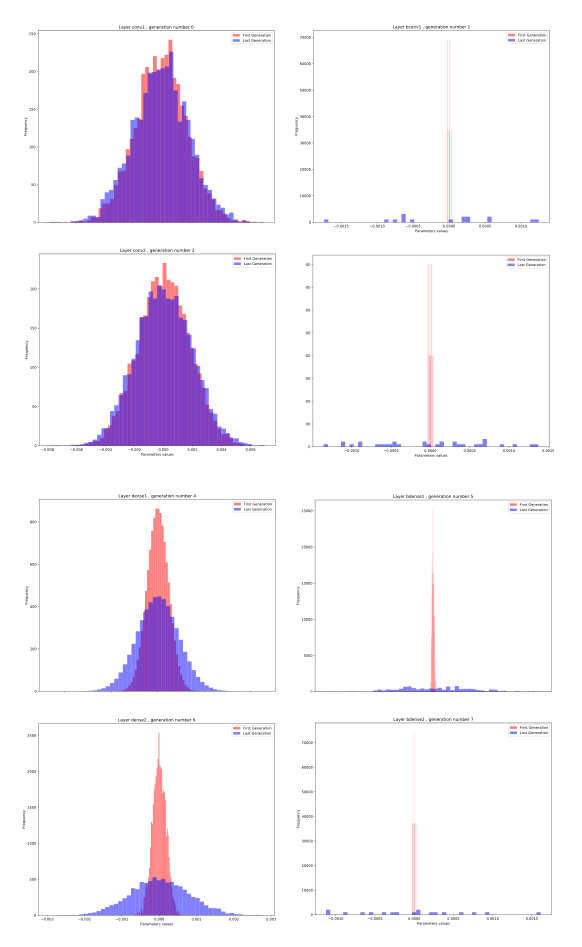
\includegraphics[width=0.95\columnwidth]{hists_best_nets.png} % Example image
	\caption{ Histogram of the networks' distribution by their scores.}
\end{figure}

\subsection{Next Steps}

Da capitolo 8 (Weighted networks) Cumulative Distributions (vedi figura 10.1) di:

\begin{itemize}
	\item figure 7-8 dendogrammi receptive fields] 
	\item link weights Q(w) vs w
	\item link weights Q(w) vs w 
	\item P(w) vs, w
	\item Sigmaw vs <w>   media e standard deviation dei pesi 
	\item P(k)  vs. k (Node strengths)  forse una misura laconica/farlocca (?!?) in questo caso ... 
	\item P(s)  vs. s 
	\item <s>(k) vs. k
	\item <Y>(k) vs. k 
\end{itemize}

\end{document}
